\section{Example of the Effects of Wakefields}

To give context to the effects that wakefields have on the both the beam and equipment with a particle accelerator, two types of wakefield/impedance driven phenomena are discussed here. The first, beam-induced heating, is an example of beam induced wakefields having an effect on the machine itself contributing to heat loads due to the energy lost by the beam and subsequently dissipated within the surrounding equipment. The second, beam instabilities, covers a number of examples of instability mechanisms that may be driven by wakefields, in particular due to the harmonic nature of particle and beam behaviour in a circular accelerator.

\subsection{Beam Induced Heating}
\label{sec:beam_induced_heating}
\subsubsection{Defining and Deriving Power Loss in Circular Accelerators}
\label{sec:power_loss}

When a charged particle interacts with an impedance it losses energy to generate the resulting wakefield. This is called the parasitic loss, and is generally defined as[ref Chao/Ng]

\begin{equation}
\Delta E = -2\pi e^{2}N_{b}\int^{\infty}_{-\infty} d\omega \left| \lambda \left( \omega \right)  \right|^{2} Z_{\parallel} \left( \omega \right)
\end{equation}

where $\Delta E$ is the energy loss per pass per particle, $e$ is the charge per particle, $N_{b}$, $\omega$ the frequency, $\lambda$ the line density of the bunch and $Z_{\parallel}$ the longitudinal impedance of the object being traversed.
																
Due to the decay of the wakefields induced by this energy loss, this energy must eventually be lost to the device causing the impedance (valid below the cutoff frequency of the machine beam pipe). Therefore we can assume that the energy loss from the particles is absorbed by the surrounding structure. Summing over all particles in a bunch we can therefore obtain a sum of the energy loss;

\begin{equation}
\Delta E_{bunch} = 2\pi \left( eN_{b}   \right)^{2} \int^{\infty}_{-\infty} d\omega \left| \lambda \left( \omega \right)  \right|^{2} Z_{\parallel} \left( \omega \right)
\end{equation}

As often we must deal with machines storing multiple bunches, for these we simply multiply the energy loss per bunch by the number of stored bunches to acquire the total energy loss per passage;

\begin{equation}
\Delta E_{bunches} = 2\pi \left( eN_{b}   \right)^{2}n_{bunch} \int^{\infty}_{-\infty} d\omega \left| \lambda \left( \omega \right)  \right|^{2} Z_{\parallel} \left( \omega \right)
\end{equation}

where $n_{bunch}$ is the number of bunches in the machine. If we assume a revolution frequency $f_{rev}$ we thus get a power loss of;

\begin{align}
P_{loss}  = & \Delta E_{bunches} f_{rev}\nonumber \\  
 = & 2\pi f_{rev} \left( eN_{b}   \right)^{2}n_{bunch} \int^{\infty}_{-\infty} d\omega \left| \lambda \left( \omega \right)  \right|^{2} Z_{\parallel} \left( \omega \right) \nonumber  \\ 
 = & 2\pi f_{rev} \left( eN_{b}   \right)^{2}n_{bunch} \int^{\infty}_{-\infty} d\omega \left| \lambda \left( \omega \right)  \right|^{2} Z_{\parallel} \left( \omega \right) \nonumber \\
 = & 2\pi f_{rev} \left( eN_{b}   \right)^{2}n_{bunch} \int^{\infty}_{-\infty} d\omega \left| \lambda \left( \omega \right)  \right|^{2} \left( \Re{}e \left( Z_{\parallel} \left( \omega\right) + \Im{}m Z_{\parallel} \left( \omega\right) \right) \right).
\end{align}
 
As $\Re{}e\left(Z_{\parallel} \left( \omega\right)\right)$ is an even function and $\Im{}m\left(Z_{\parallel} \left( \omega\right)\right)$ is an odd function, we see that

\begin{equation}
P_{loss}   =  \omega_{rev} \left( eN_{b}   \right)^{2}n_{bunch} \int^{\infty}_{0} 2 d\omega \left| \lambda \left( \omega \right)  \right| ^{2}  \Re{}e \left( Z_{\parallel} \left( \omega\right)  \right).
\label{eqn:power_loss_omega}
\end{equation}

Next we make a change of the variable of integration $\omega = n_{bunch}\omega_{rev}$;

\begin{equation}
P_{loss}   =  \omega_{rev} \left( eN_{b}   \right)^{2}n_{bunch}^{2} \int^{\infty}_{0} 2 d\omega_{rev} \left| \lambda \left( \omega_{rev}n_{bunch} \right)  \right|^{2}  \Re{}e \left( Z_{\parallel} \left( \omega_{rev}n_{bunch}\right)  \right).
\end{equation}

We can subsequently change to a sum formalism to obtain

\begin{equation}
P_{loss} = \left( \omega_{rev}eN_{b}n_{bunch}  \right)^{2} \displaystyle\sum\limits_{p = 0}^{\infty} \left( 2 \left| \lambda \left(p \omega_{rev}n_{bunch} \right)  \right|^{2}  \Re{}e \left( Z_{\parallel} \left(p \omega_{rev}n_{bunch}\right) \right) \right) \label{ean:heating-gen}
\end{equation}

where $\omega_{0} = 2\pi f_{0}$, $f_{0} = \frac{1}{\tau_{b}}$ and $\tau_{b}$ is the bunch spacing.

\subsubsection{Longitudinal Beam Profiles}

As shown by the derivations in Section~\ref{sec:power_loss}, asides from the longitudinal impedance of the device under consideration the longitudinal profile of the circulating bunches also contributes to the power loss in the machine. In past works it has generally been assumed that bunches in accelerators have a Gaussian profile [ref Sacherer/Grudiev/Laclare](seen in Eqn.~\ref{eqn:gauss}, where $4\sigma_{z} = t_{b}$, $t_{b}$ is the bunch length) when approaching the analytical treatment of beam instabilities, both single-bunch and multi-bunch. Recent measurements of the power spectrum of particle beams, especially in the LHC [ref theo/phillipe] have shown characteristics that the Gaussian profile does not predict, for example the high frequency secondary peak as seen in Fig.~\ref{fig:measured_gauss}. To make more realistic predictions of heat loss due to beam impedance in the machine it is thus necessary to find bunch profiles which reproduce this behaviour.

\begin{equation}
\lambda \left( t \right) = e^{\frac{-t^{2}}{2\sigma^{2}}}
\label{eqn:gauss}
\end{equation}

\begin{figure}
\subfigure[]{
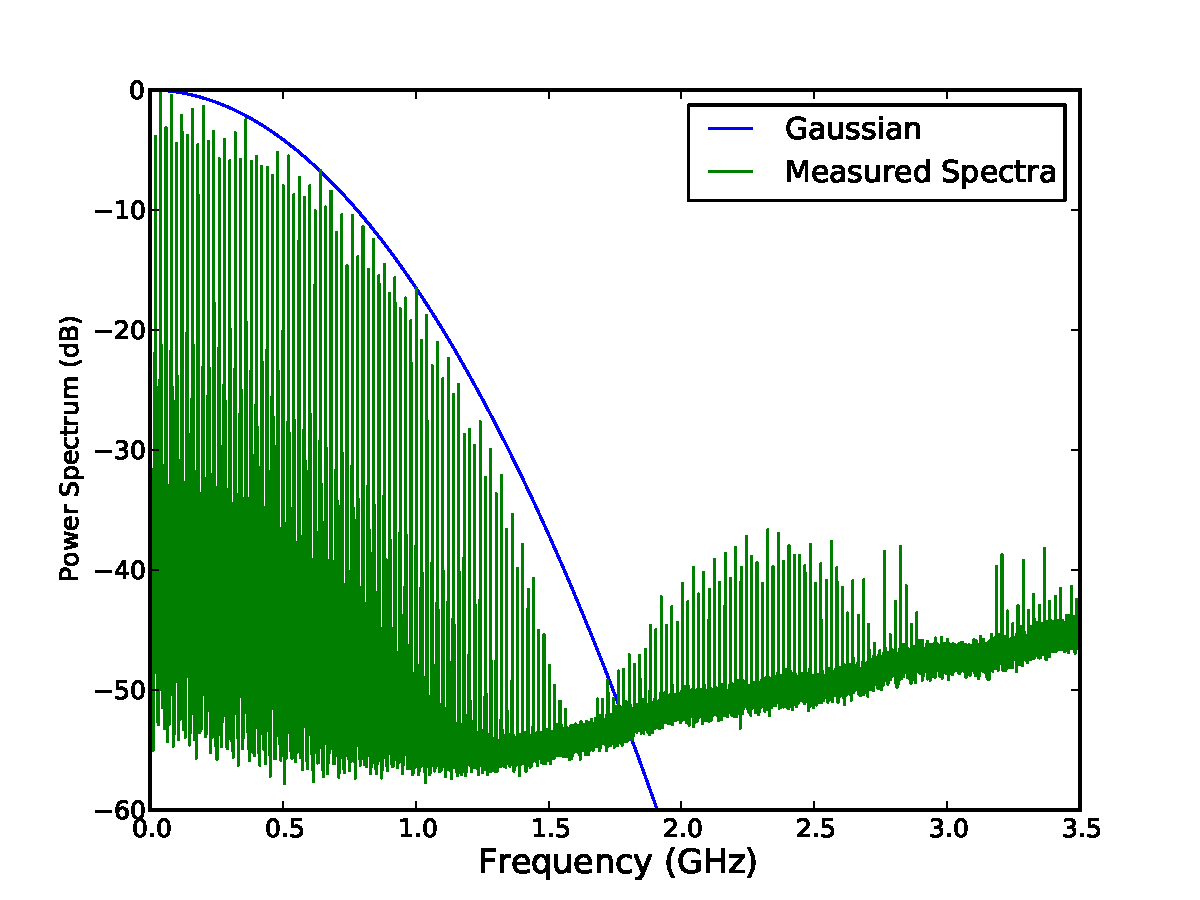
\includegraphics[width=0.45\textwidth]{Wakefields_and_Impedances/figures/beam_spectra_power_gauss_meas_12ns.pdf}
\label{fig:gauss_meas_freq}
}
\subfigure[]{
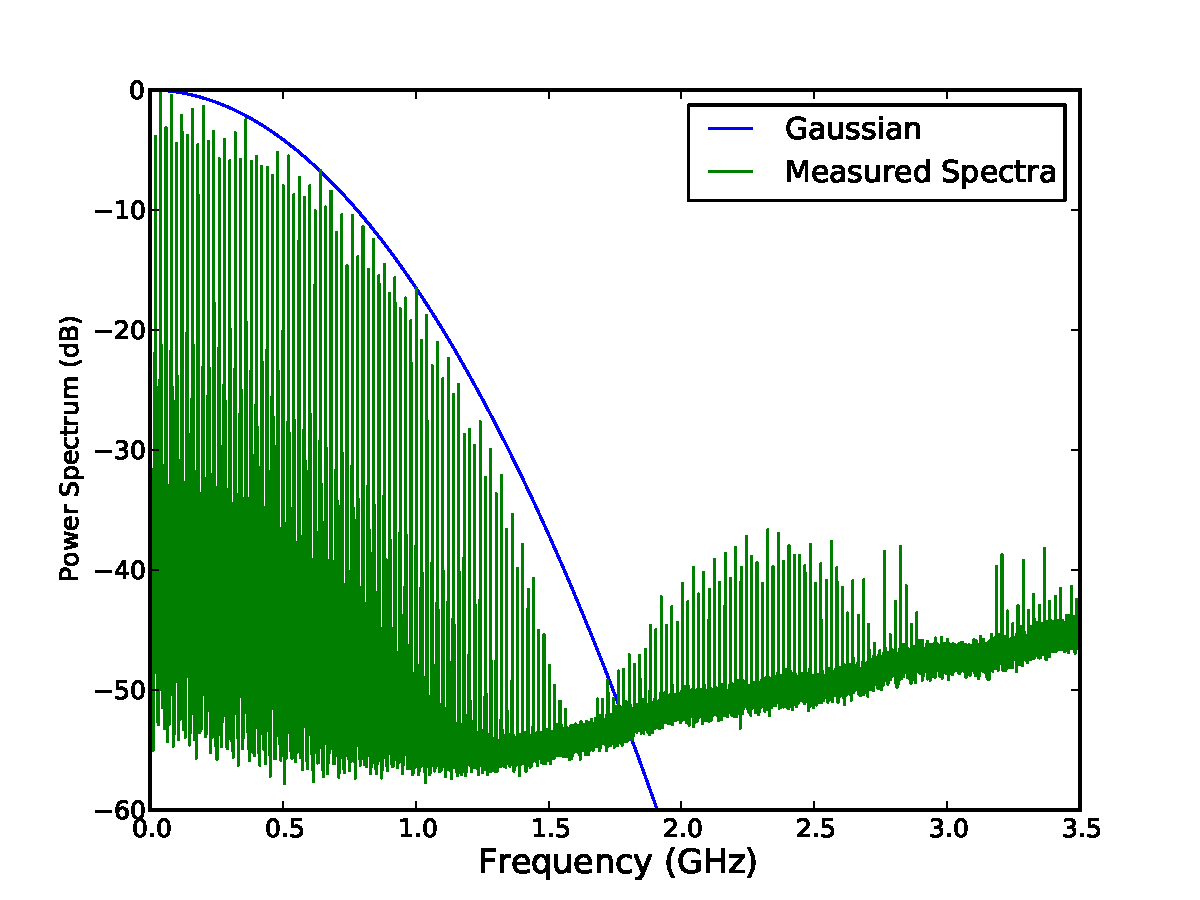
\includegraphics[width=0.45\textwidth]{Wakefields_and_Impedances/figures/beam_spectra_power_gauss_meas_12ns.pdf}
\label{fig:gauss_meas_time}
}
\caption{A comparison of \ref{fig:gauss_meas_freq} a measured beam power spectrum and a gaussian bunch of the same bunch length in the frequency domain and \ref{fig:gauss_meas_time} the resulting time domain beam profile. The gaussian has a bunch length (4$\sigma_{z}$ = 1.2ns) }
\label{fig:measured_gauss}
\end{figure}

A number of different longitudinal bunch profiles have been investigated in the past. Here we shall look at 3 other bunch profiles; a parabolic line density (see Eqn.~\ref{eqn:para_profile}), cos$^{2}$ (see Eqn.~\ref{eqn:cos_profile}), water-bag (see Eqn.~\ref{eqn:water_bag_profile}).

\begin{equation}
A\left( t \right) = \int^{\infty}_{-\infty} \lambda \left( \omega \right) e^{j\omega t} d\omega = 
\begin{cases}1-\left( \frac{2t} {t_{b}} \right)^{2} &\textrm{if $| t/2 | \leq t_{b}$}\\
0								&\textrm{if $| t/2 | > t_{b}$}
\end{cases}
\label{eqn:para_profile}
\end{equation}

\begin{equation}
A\left( t \right) = \int^{\infty}_{-\infty} \lambda \left( \omega \right) e^{j\omega t} d\omega = 
\begin{cases}
cos^{2}\left( \frac{\pi t} {t_{b}} \right) &\textrm{if $| t/2 | \leq t_{b}$}\\
0								&\textrm{if $| t/2 | > t_{b}$}
\end{cases}
\label{eqn:cos_profile}
\end{equation}

\begin{equation}
A\left( t \right) = \int^{\infty}_{-\infty} \lambda \left( \omega \right) e^{j\omega t} d\omega = 
\begin{cases}
\sqrt{1-\left( \frac{2t}{t_{b}}\right)^{2}} &\textrm{if $| t/2 | \leq t_{b}$}\\
0								&\textrm{if $| t/2 | > t_{b}$}
\end{cases}
\label{eqn:water_bag_profile}
\end{equation}

The comparison of these bunch profiles in the time domain are shown in Fig.~\ref{fig:time_bunch_profiles}. Note all bunch currents are normalised to their peak value. The corresponding current and power spectrums are shown in Fig.~\ref{fig:freq_dom_prof}. There are several things to note about these spectra; firstly that the non-infinite distribution of the non-gaussian bunch profiles gives rise to a number of high frequency lobes in the power spectrum, and secondly the interval of these nodes depends heavily on the bunch profile.

\begin{figure}
\begin{center}
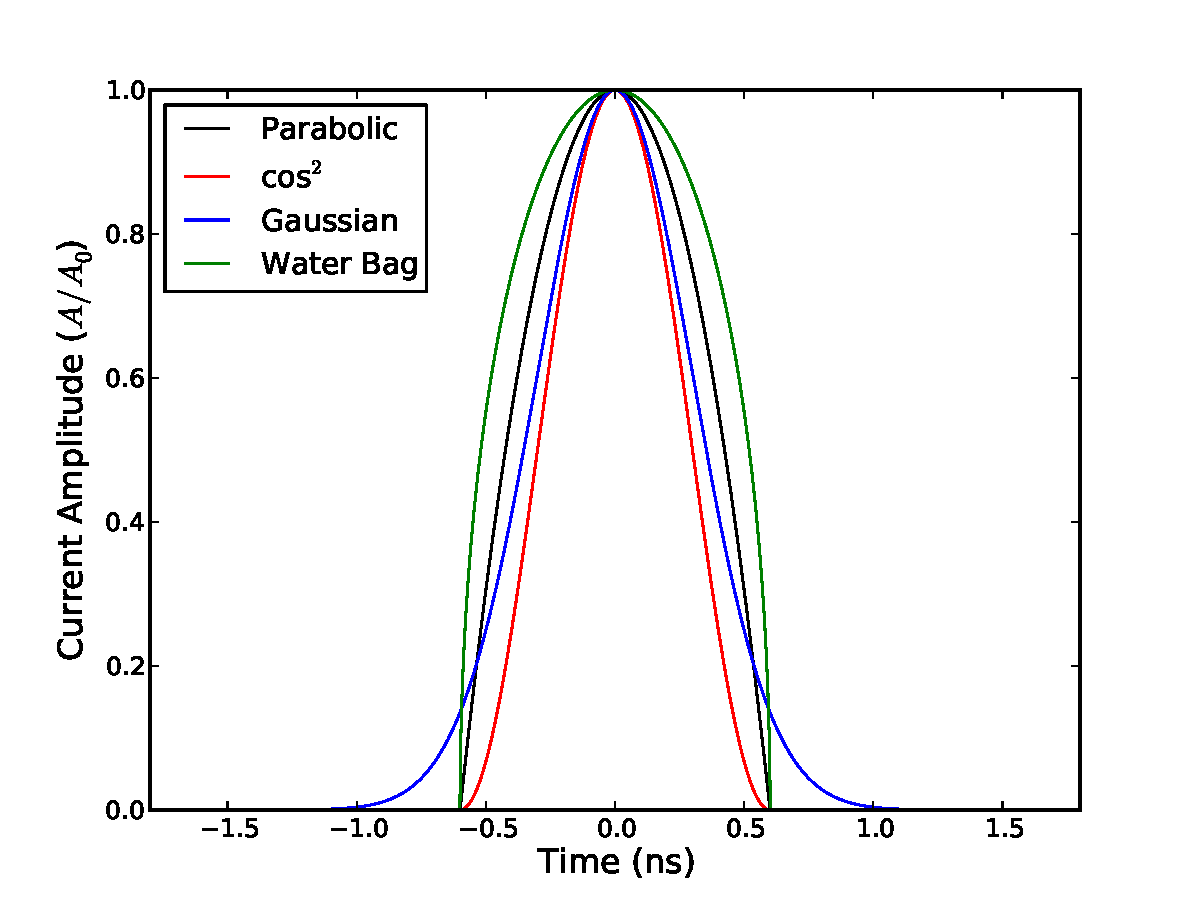
\includegraphics[width=0.65\textwidth]{Wakefields_and_Impedances/figures/bunch_profile_12ns.pdf}
\end{center}
\label{fig:time_bunch_profiles}
\caption{The longitudinal bunch profile of a number of bunch distributions. Note that all of them are normalised to have a peak bunch current of 1. For the gaussian distribution the bunch length is the 4$\sigma$ value. The bunch length $\tau_{b} = 1.2ns$}
\end{figure}

\begin{figure}
\subfigure[]{
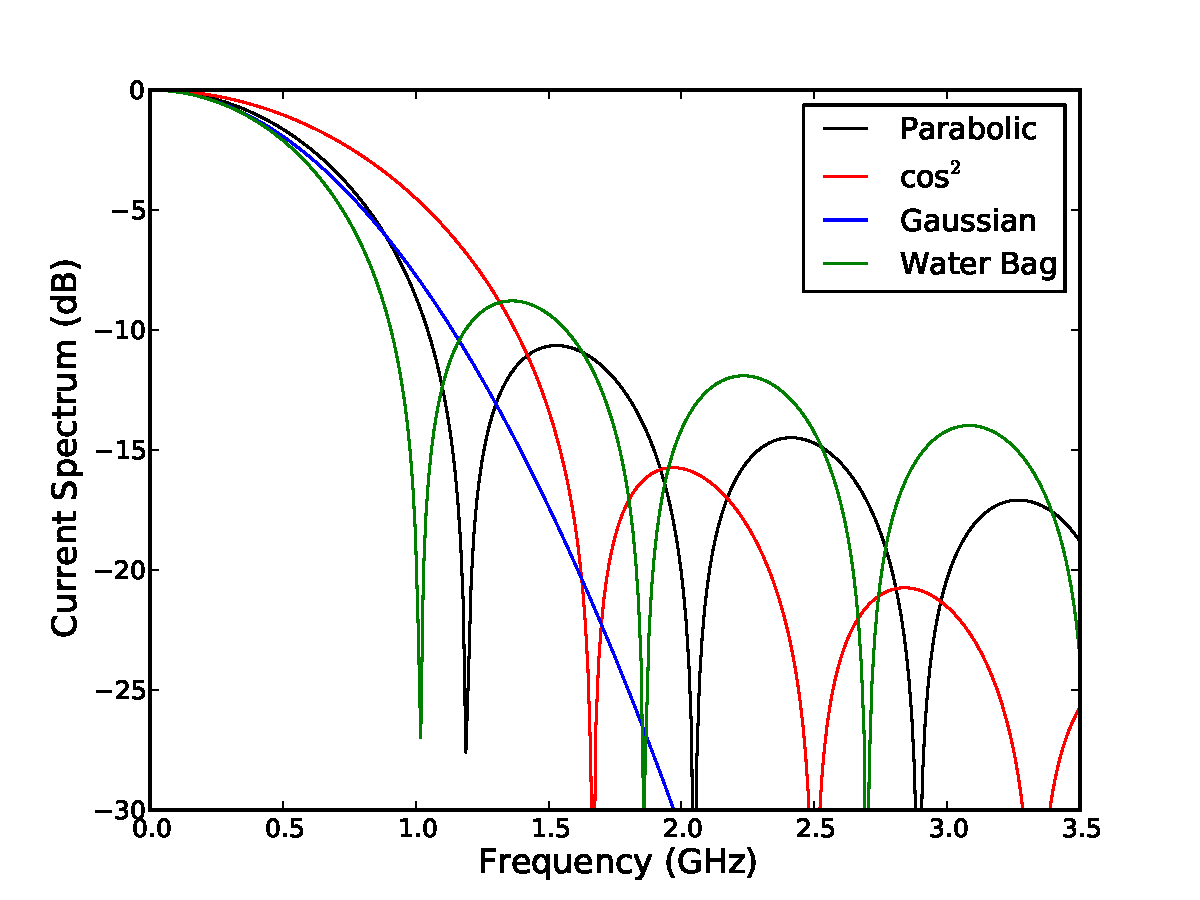
\includegraphics[width=0.45\textwidth]{Wakefields_and_Impedances/figures/current_spectrum_12ns.pdf}
\label{fig:current_spec}
}
\subfigure[]{
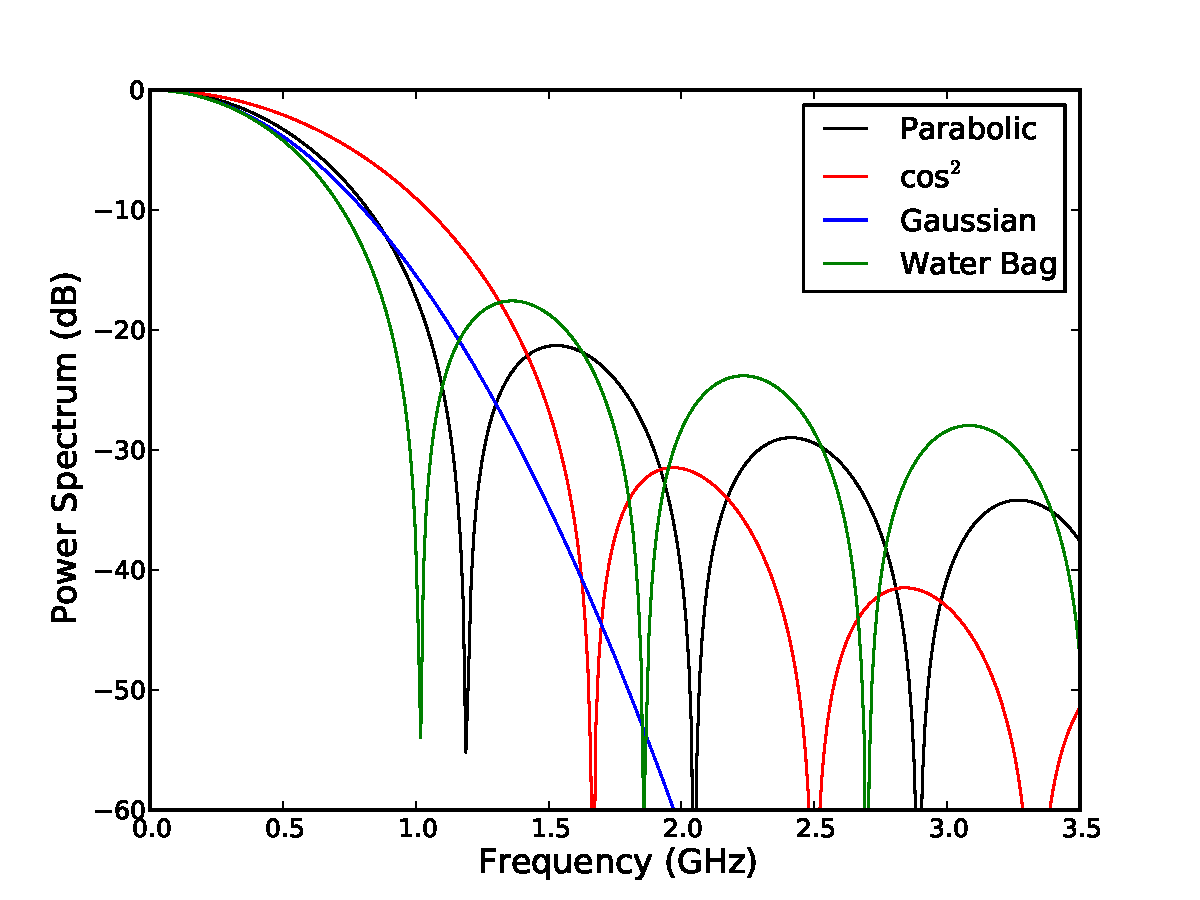
\includegraphics[width=0.45\textwidth]{Wakefields_and_Impedances/figures/power_spectrum_12ns.pdf}
\label{fig:power_spec}
}
\label{fig:freq_dom_prof}
\caption{The frequency domain \ref{fig:current_spec} current spectrum and \ref{fig:power_spec} power spectrum for a number of different bunch profiles with a bunch length $\tau_{b} = 1.2ns$.}
\end{figure}

To illustrate more clearly the effect of changing the bunch length on the power spectrum, a number of bunch profiles and the corresponding power spectra with different bunch lengths are shown below. Firstly, consider a gaussian bunch profile. It can be seen in Fig.~\ref{fig:diff_bunch_len_gauss} that by increasing the bunch length that the magnitude at high frequencies is decreased quite substantially as the bunch length increases. If we consider a finite bunch profile (non-gaussian), we note that we have high frequency lobes. The peak frequency of these lobes depends on the bunch length, as illustrated using a parabolic bunch profile for bunch lengths $\tau_{b} = 1ns, 1.2ns, 1.4ns$ in Fig.~\ref{fig:diff_bunch_len_para}. As the bunch length is increased the lobes move to lower frequencies, and the width of the first branch decreases, as seen for the gaussian bunch. Similar behaviour is observed with the cos$^{2}$ and water-bag bunch profiles.

\begin{figure}
\subfigure[]{
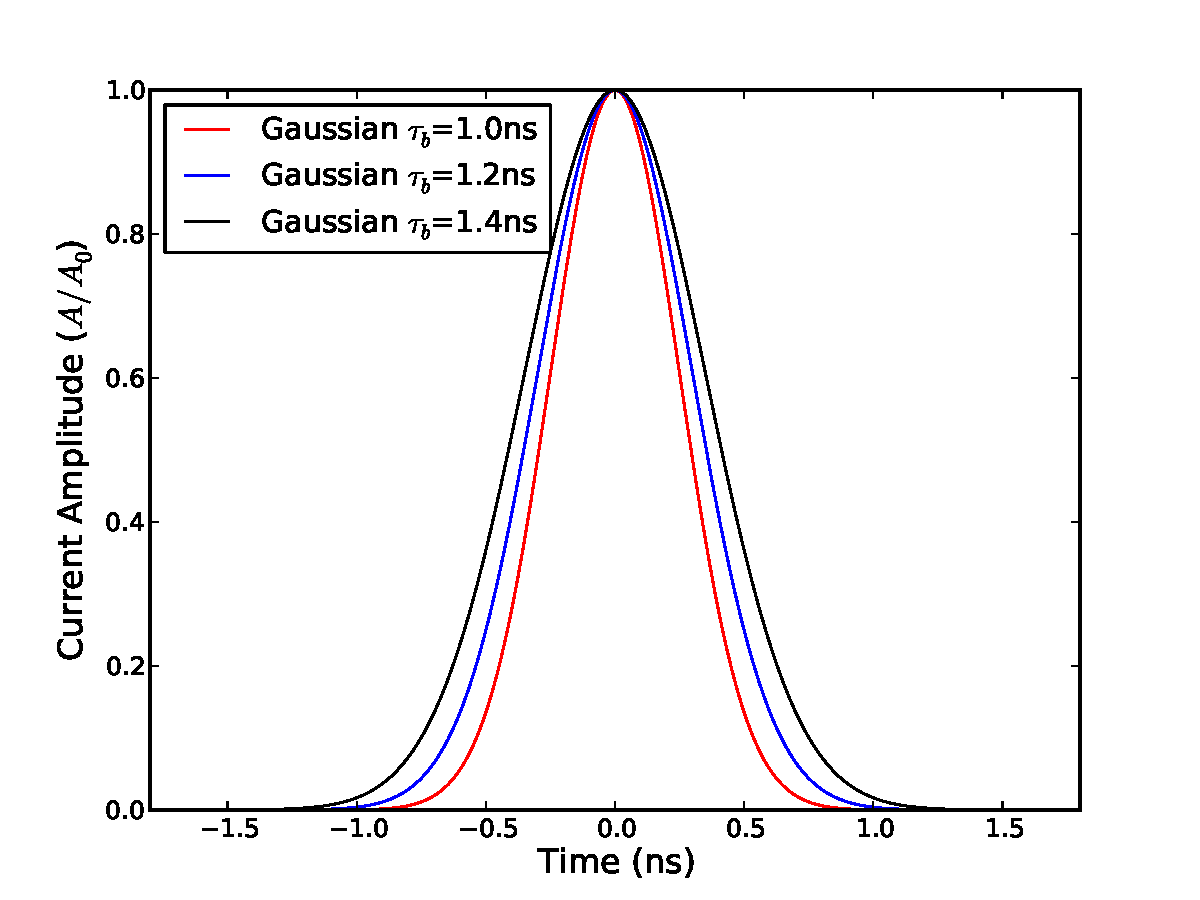
\includegraphics[width=0.45\textwidth]{Wakefields_and_Impedances/figures/gaussian_time_dom_diff_lengths.pdf}
\label{fig:change_len_time_gauss}
}
\subfigure[]{
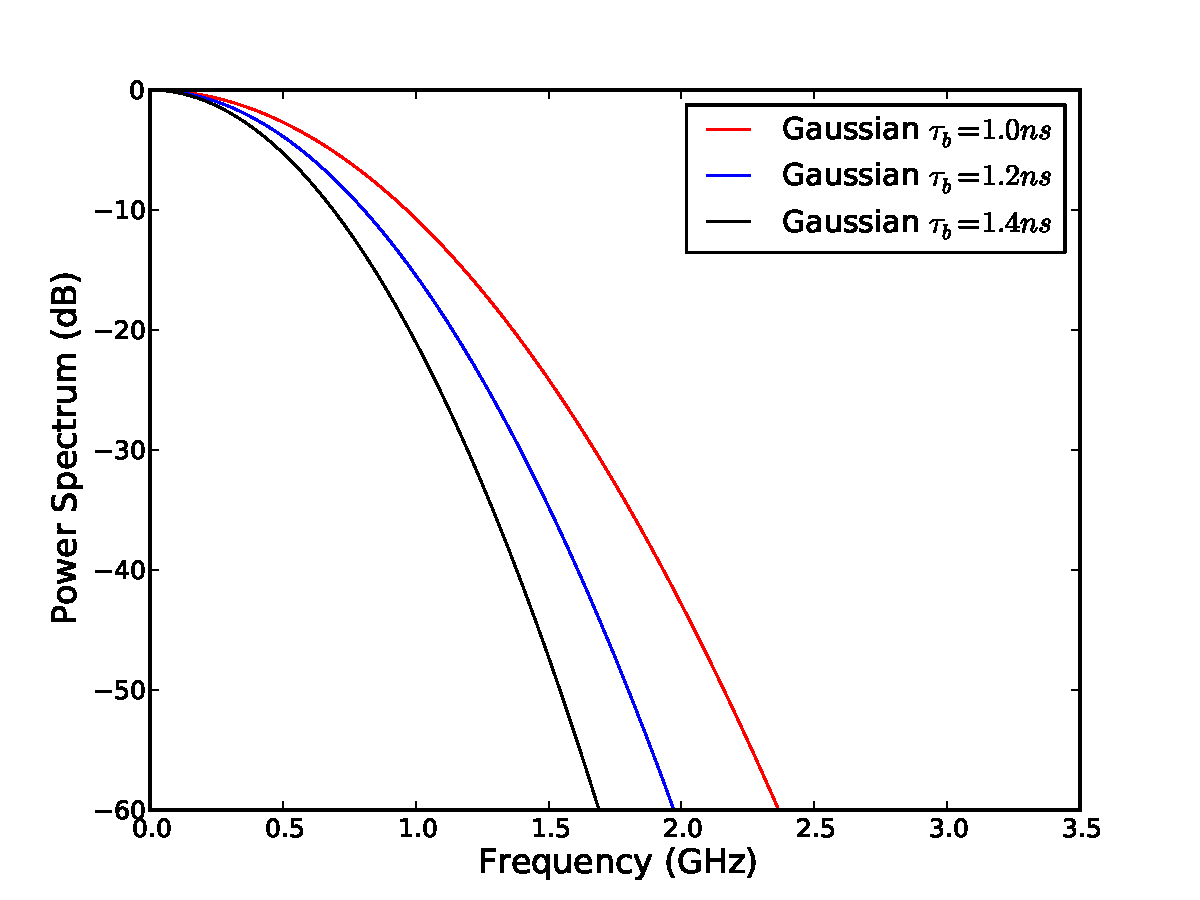
\includegraphics[width=0.45\textwidth]{Wakefields_and_Impedances/figures/gaussian_power_spec_diff_lengths.pdf}
\label{fig:change_len_freq_gauss}
}
\caption{\ref{fig:change_len_time_gauss} The longitudinal profile and the \ref{fig:change_len_freq_gauss} associated bunch power spectrum for a number of bunch lengths assuming a gaussian bunch profile.}
\label{fig:diff_bunch_len_gauss}
\end{figure}

\begin{figure}
\subfigure[]{
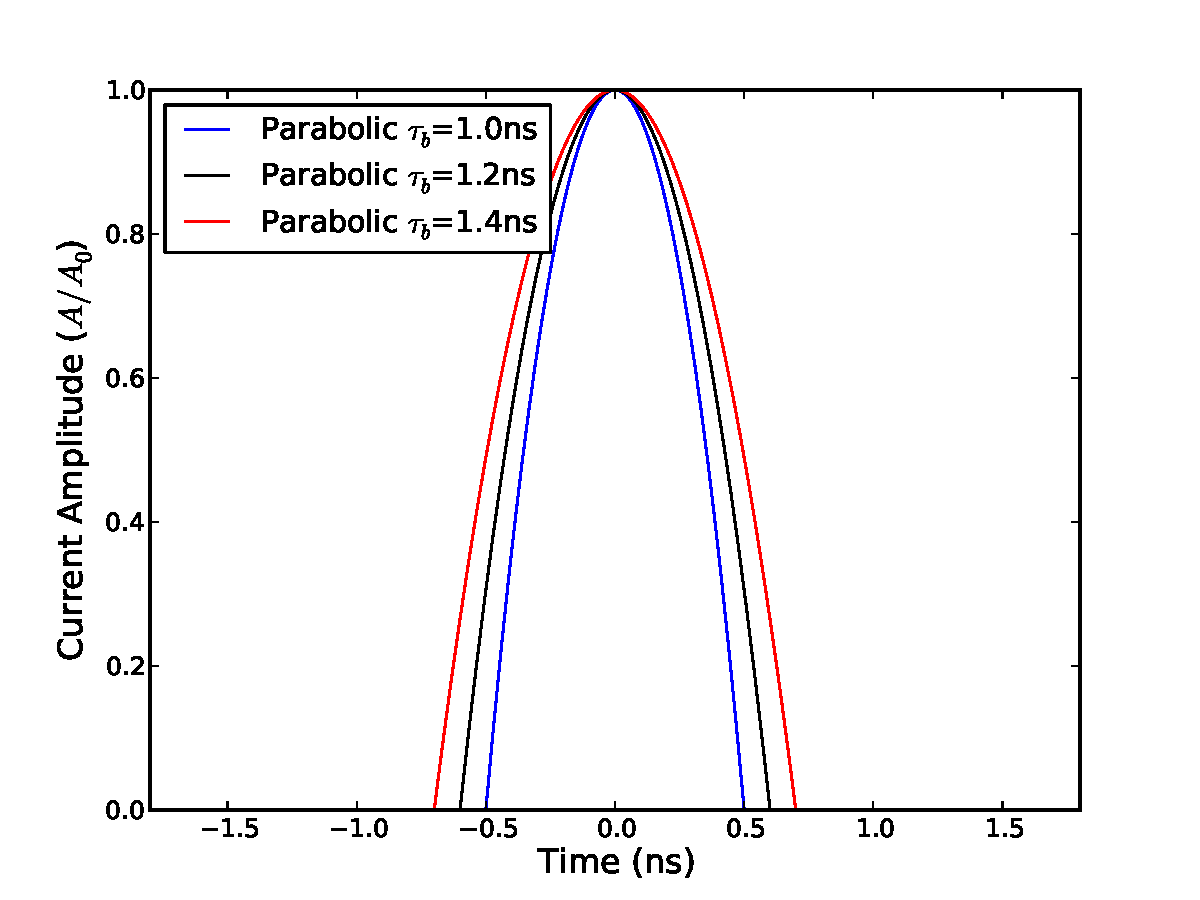
\includegraphics[width=0.45\textwidth]{Wakefields_and_Impedances/figures/current_amp_para_change.pdf}
\label{fig:change_len_time_para}
}
\subfigure[]{
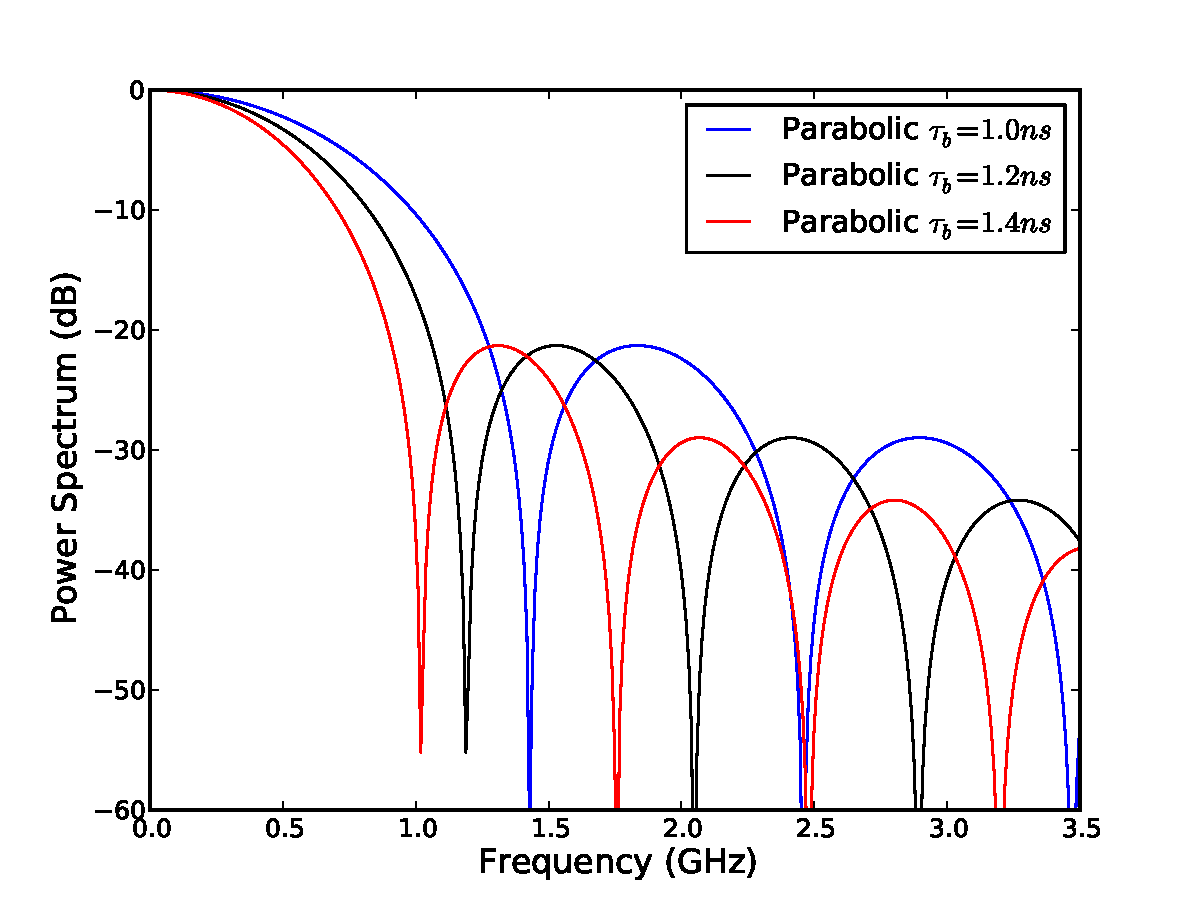
\includegraphics[width=0.45\textwidth]{Wakefields_and_Impedances/figures/freq_power_para_change.pdf}
\label{fig:change_len_freq_para}
}
\caption{\ref{fig:change_len_time_para} The longitudinal profile and the \ref{fig:change_len_freq_para} associated bunch power spectrum for a number of bunch lengths assuming a parabolic bunch profile.}
\label{fig:diff_bunch_len_para}
\end{figure}

Finally, a comparison of a measured bunch power spectra and the analytical power spectra is shown in Fig.~\ref{fig:power_all}. It can be seen that whilst it is possible to replicate some of the properties of the measured spectrum, an exact replication is non-trivial. Further investigation into the appropriate bunch profile is ongoing.

\begin{figure}
\begin{center}
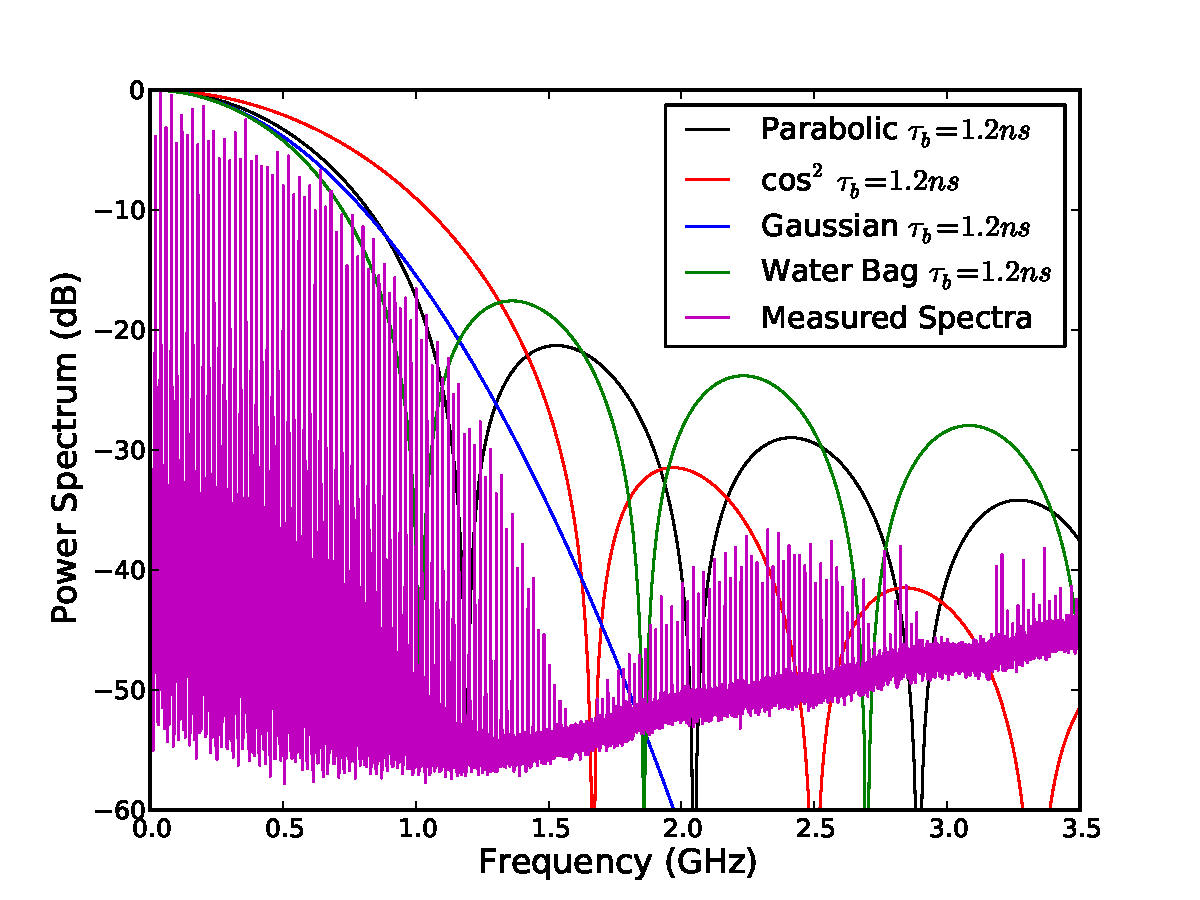
\includegraphics[width=0.65\textwidth]{Wakefields_and_Impedances/figures/beam_spectra_power_12ns.pdf}
\end{center}
\label{fig:power_all}
\caption{A comparison of a measured beam power spectrum and a number of analytical bunch profiles assuming a bunch length of 1.2ns.}
\end{figure}



% Introduce a number of longitudinal profiles in time domain - gaussian, parabolic line density, cos^2, water bag - comments of realism (gaussian being infinite) - truncated gaussian
% Comparison in the frequency domain - firstly gaussian compared to truncated gaussian - infinite tails reduce the magnitude of the higher frequency components and lobe
% Gaussian, parabolic, cos^2 - all with the same bunch length
% Using the above examples try using a number of different bunch lengths to illustrate how they change (gaussian - just extends further, parabolic, cos^2 lobe frequency changes)
% Finally - comparison to measured spectra to illustrate changes in bunch length and frequency components as bunch is ramped and squeezed

\subsubsection{Beam induced heating due to a low Q impedance}

For an impedance with a characteristic Q that is small (Q $<$ 10), it can be seen that the impedance peak will interact substantially with a number of beam harmonics (see Fig.~\ref{fig:low_q_harmonics}) due to the broad frequency range it occupies.

\begin{figure}
\begin{center}
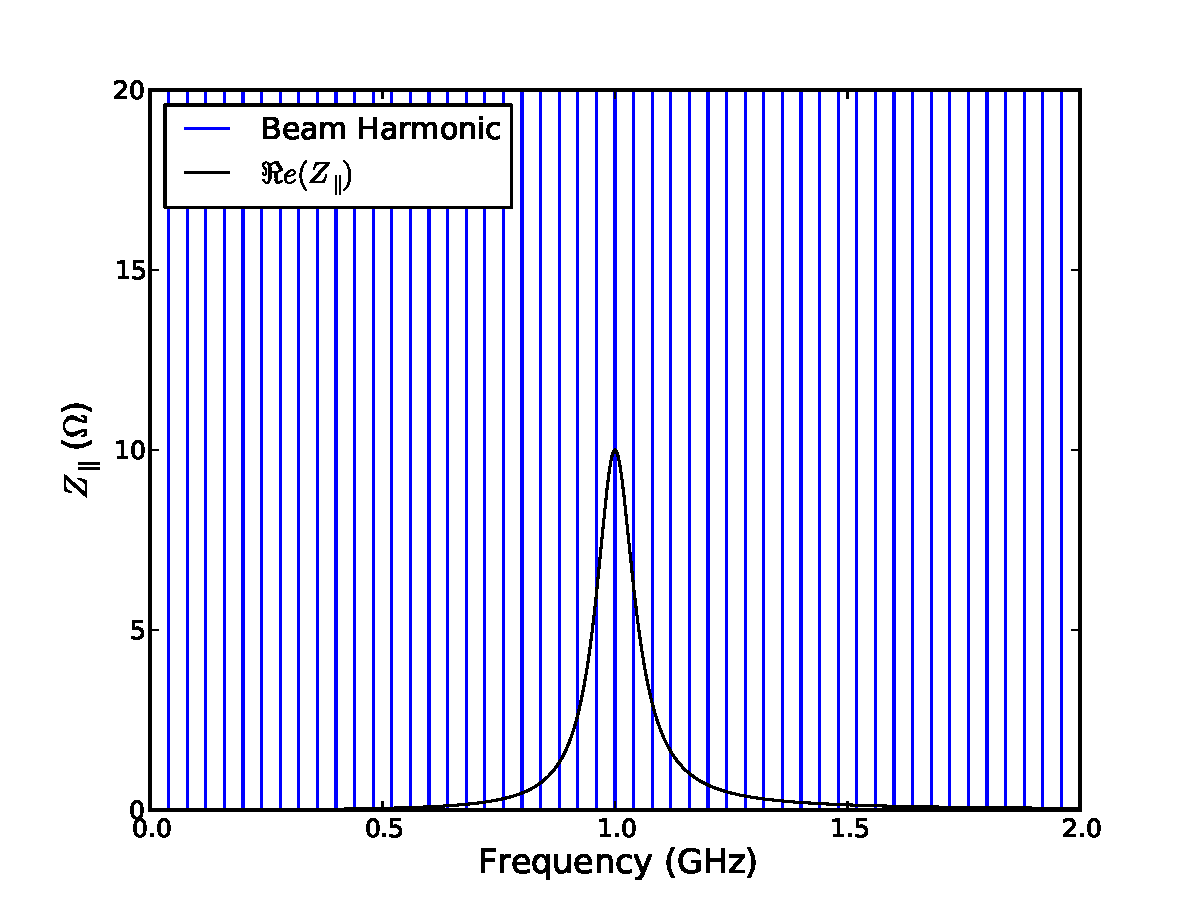
\includegraphics[width=0.65\textwidth]{Wakefields_and_Impedances/figures/low_q_10_resonance_beam_harmonics.pdf}
\end{center}
\label{fig:low_q_harmonics}
\caption{The beam harmonics of a beam with a bunch spacing of 25ns overlayed on the real component of the longitudinal impedance an example of a low Q impedance ($R_{s}=10\omega$, Q = 10, $f_{res}=1GHz$). The blue lines represent the frequency of a beam harmonic, not necessarily the magnitude of the power spectrum at that point. Note that a number of beam harmonics overlay non-zero impedance values.}
\end{figure}

Further investigation of the longitudinal beam spectrum reveals that there is significant structure between the major harmonics (which are due to the bunch spacing of the beam) which can be attributed to the other time structures of the beam, for example the bunch train spacing, or the interval between the pilot bunch train and the subsequent bunch train. As such the treatment of the estimation of beam losses requires a broad spectrum approach. If we consider Eqn.\ref{eqn:power_loss_omega} we see that we can treat the power losses in an integral form. We can observe a number of properties using this assumption. The power loss is proportional to the beam properties in the following manner:

\begin{enumerate}
\item{$P_{loss} \propto N^{2}$}
\item{$P_{loss} \propto n_{bunch}$}
\end{enumerate}

\subsubsection{Beam induced heating due to a high Q impedance}

In contrast to the overlap of the beam spectrum with a low Q impedance, for a high Q impedance only one beam harmonic lies upon the resulting impedance to any significant quantity. This is illustrated in Fig~\ref{fig:high_q_harmonics} If we consider Eqn \ref{eqn:heating-gen} and consider the situation where

\begin{equation}
\left( 2 \left| \lambda \left(p \omega_{rev}n_{bunch} \right)  \right|^{2}  \Re{}e \left( Z_{\parallel} \left(p \omega_{rev}n_{bunch}\right) \right) \right) = 
\begin{cases}
\left( 2 \left| \lambda \left( \omega_{res} \right)  \right|^{2}  \Re{}e \left( Z_{\parallel} \left( \omega_{res} \right) \right) \right) &\textrm{if $p \omega_{rev} n_{bunch} = \omega_{res}$}\\
0								&\textrm{if $p \omega_{rev} n_{bunch} != \omega_{res}$}
\end{cases}
\label{eqn:single_harmonic_profile}.
\end{equation}

\begin{figure}
\begin{center}
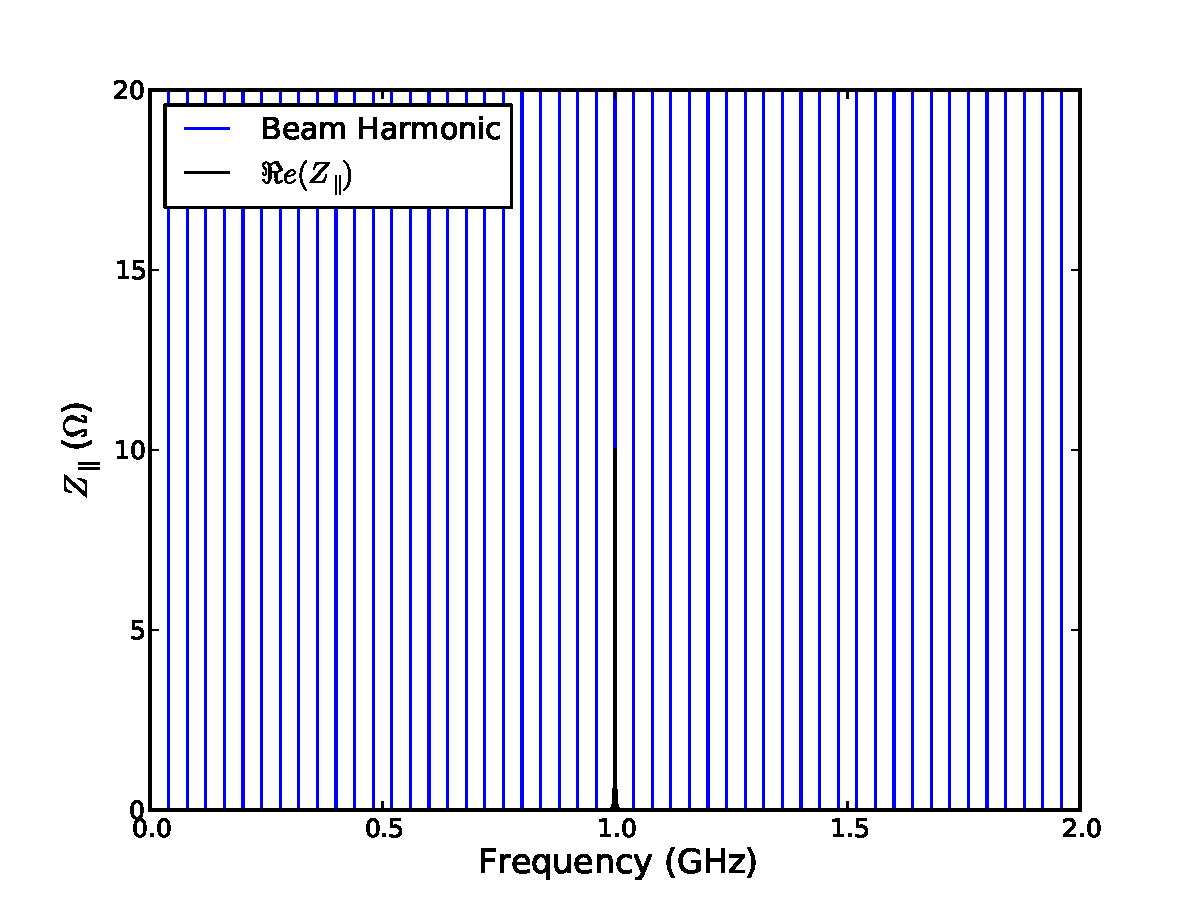
\includegraphics[width=0.65\textwidth]{Wakefields_and_Impedances/figures/high_q_1000_resonance_beam_harmonics.pdf}
\end{center}
\label{fig:high_q_harmonics}
\caption{The beam harmonics of a beam with a bunch spacing of 25ns overlayed on the real component of the longitudinal impedance an example of a high Q impedance ($R_{s}=10\omega$, Q = 1000, $f_{res}=1GHz$). The blue lines represent the frequency of a beam harmonic, not necessarily the magnitude of the power spectrum at that point. Note that only a single beam harmonic overlays a non-zero impedance values.}
\end{figure}

It can then be seen that Eqn~\ref{eqn:heating-gen} simplifies to

\begin{equation}
P_{loss} = \left( \omega_{rev}eN_{b}n_{bunch}  \right)^{2}  \left( 2 \left| \lambda \left( \omega_{res} \right)  \right|^{2}  \Re{}e \left( Z_{\parallel} \left(\omega_{res} \right) \right) \right). 
\label{ean:heating-high-q}
\end{equation}

The following properties can subsequently be seen as a result:

\begin{enumerate}
\item{$P_{loss} \propto N^{2}$}
\item{$P_{loss} \propto n_{bunch}^{2}$, provided that the resonant frequency of the resonance continues to coincide with a beam harmonic.}
\end{enumerate}

\subsubsection{Some Examples of the Beam-Induced Heating}

In this section we shall illustrate some important factors that have been covered in previous sections. In particular, the interaction of different bunch profiles at different bunch lengths with an example cavity resonance will be covered in some detail to illustrate how the estimated heating can change drastically depending on higher frequency lobes in the beam current spectrum. In addition, the heating due to two particle beams in the same vacuum chamber shall be briefly covered for interest.

\subsubsection{The Effect of Bunch Length on Power Loss}

As can be seen in Figs.~\ref{fig:freq_dom_prof} and \label{fig:diff_bunch_len_para}, the bunch profile and the bunch length can significantly alter the magnitude of the beam current at higher frequencies. To illustrate this, let us consider two resonant impedances, one broadband $Z_{bb}$ and one narrow band $Z_{nb}$ impedance, characterised by having a low-$Q$ and a high-$Q$ respectively. Both impedances shall have the same resonant shunt impedance $R_{s} = 100\Omega$. The broadband impedance shall have a $Q_{bb}=1$, and the narrow band impedance $Q_{nb}=1000$. The resonant frequency will be changed to illustrate effects in different regimes of the bunch length and of different bunch profiles.

We shall use the gaussian bunch profile and the $cos^{2}$ bunch profile for these examples. The gaussian is useful to illustrate the effect of just the changing bunch length, and the $cos^{2}$ due to the presence of a high frequency lobe in it's frequency domain current spectrum. The $cos^{2}$ frequency domain current profile is given by

\begin{equation}
I \left( \omega \right) = \frac{sin \left( \omega \tau_{b}/2 \right)}{ \omega \tau_{b}/2 \left[ 1 - \left(  \omega \tau_{b}/2 \right)^{2}  \right]}.
\end{equation}

First we shall consider a narrowband impedance which has a resonant frequency $\omega_{0} =2GHz$ which falls upon a beam harmonic such that $\omega_{0}=n\omega_{rev}$ where n is an integer. It should be noted that for other cases the contribution of these sources of heating is negligible due to the small beam current at this frequency. There are two extreme cases; that of  $\omega_{0} \gg 1/\tau_{b}$, in which it can be seen that the current spectrum will be negligible at the frequency of the impedance, and $\omega_{0} \ll 1/\tau_{b}$ where the beam current spectrum is essentially the same as the DC spectral component. The transition in this intervening regime is shown in Fig~\ref{fig:bunch_length_heat_narrow}, assuming a bunch current of 1A. It can be seen that in this case the heating falls drastically as the bunch length increases.

\begin{figure}
\begin{center}
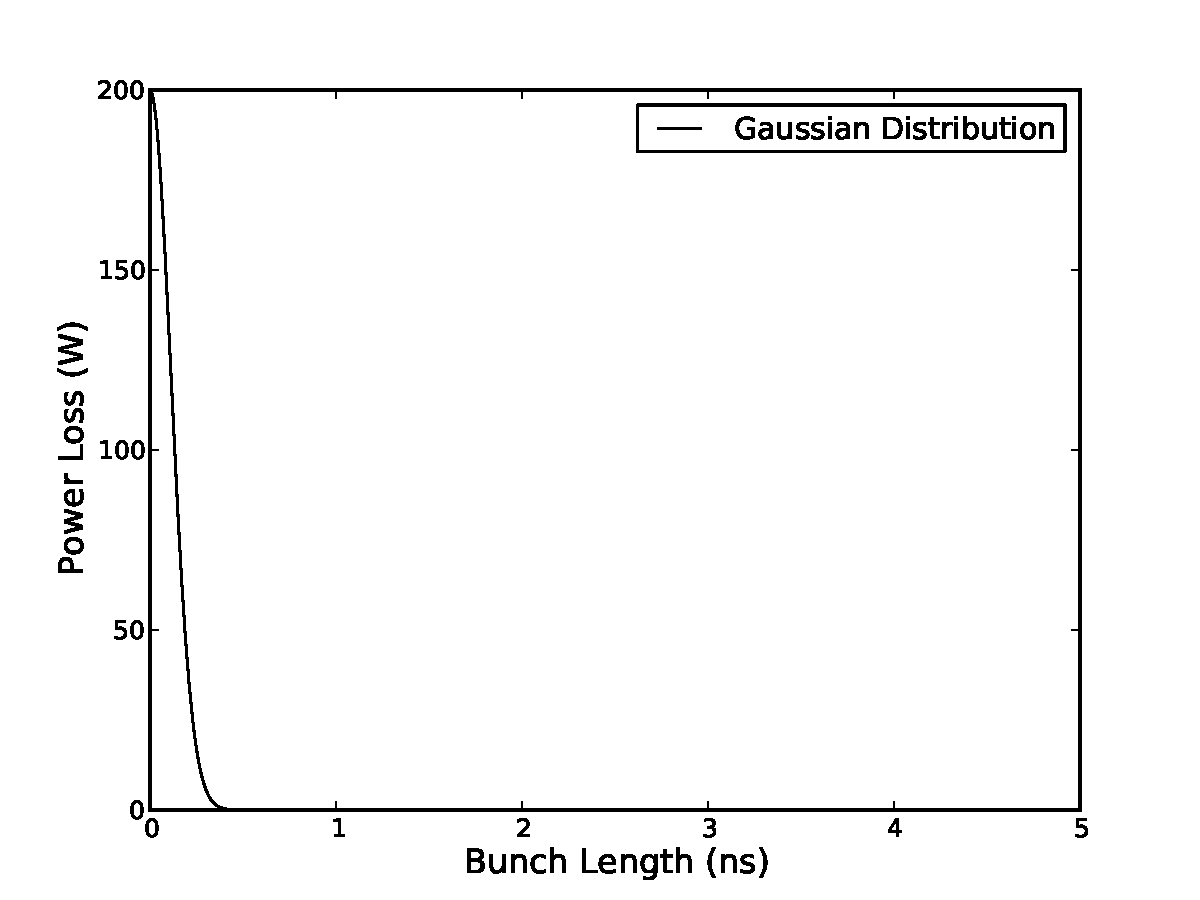
\includegraphics[width=0.8\textwidth]{Wakefields_and_Impedances/figures/heating_narrowband_gauss_bunch_length.pdf}
\end{center}
\label{fig:bunch_length_heat_narrow}
\caption{The change in power loss due to a narrow band resonance characterised by $\omega_{0} = 2GHz$, $R_{s} = 100\Omega$, $Q = 1000$ with a gaussian bunch distrbution of different lengths.}
\end{figure}

If we instead consider a cos$^{2}$ distribution we instead see the effect of the secondary lobes in the beam current spectrum. The power loss with bunch length is shown in Fig.~\ref{fig:bunch_length_heat_narrow_cos} in comparison to that of the gaussian profile. The beam power spectrum for a number of different bunch lengths are shown with the real component of the longitudinal impedance in Fig.~\ref{fig:imp_profile_cos}. Here it can be clearly seen that the intersection of the secondary lobe with the resonant impedance causes a peak in the power lost by the beam, highlighting the neccessity to be aware of the resonant frequencies of resonant impedances with relation to the beam harmonics.


\begin{figure}
\subfigure[]{
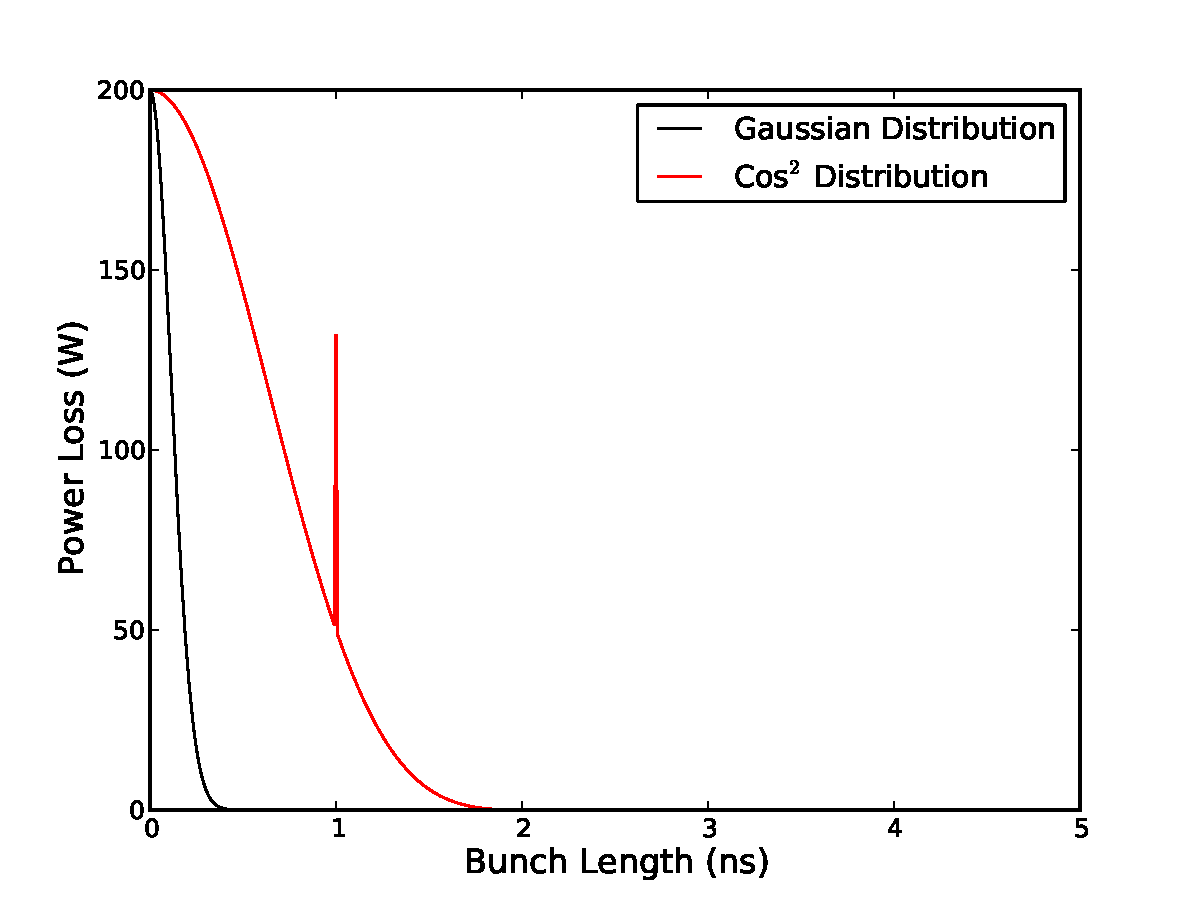
\includegraphics[width=0.5\textwidth]{Wakefields_and_Impedances/figures/heating_narrowband_gausscos_bunch_length.pdf}
\label{fig:long_imp_narrow_current}
}
\subfigure[]{
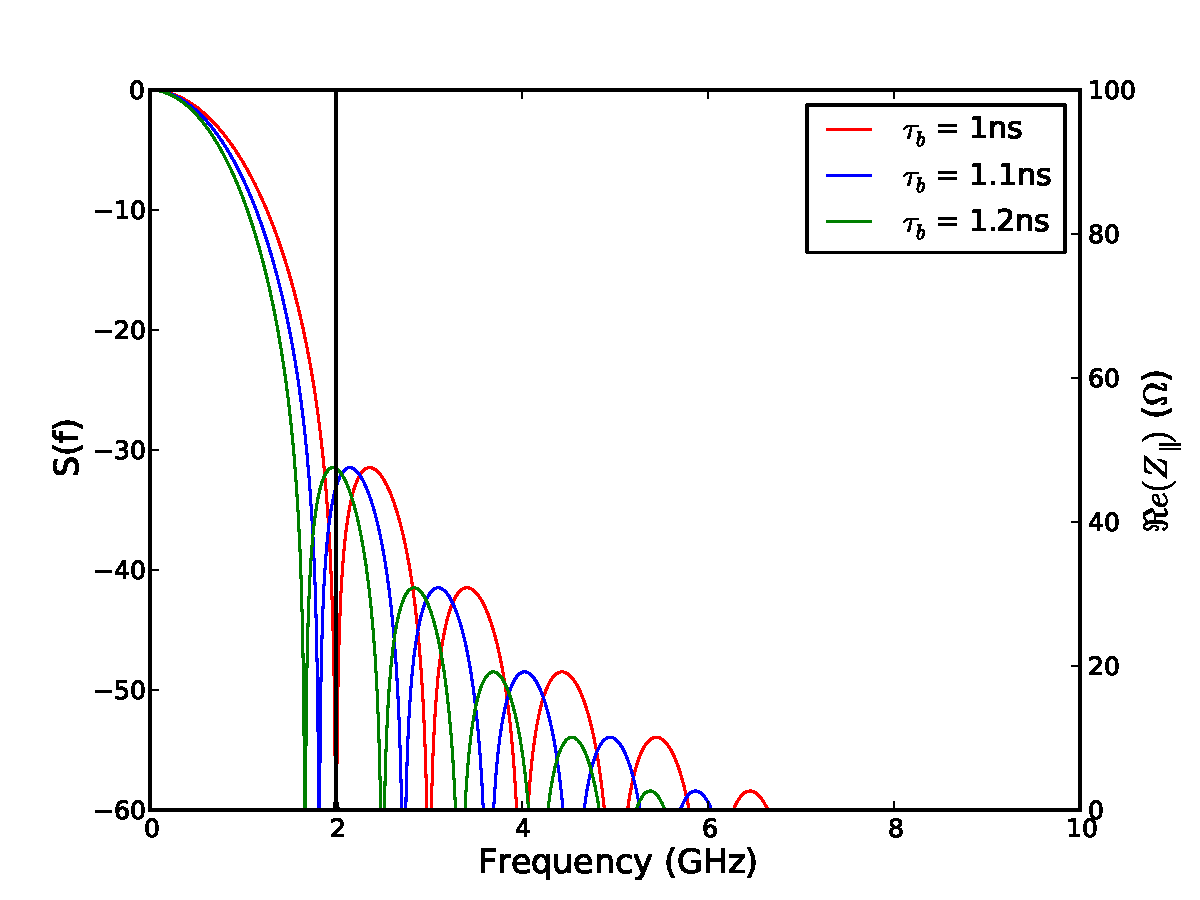
\includegraphics[width=0.5\textwidth]{Wakefields_and_Impedances/figures/impedance_and_power_cos_res.pdf}
\label{fig:imp_profile_cos}
}
\caption{\ref{fig:long_imp_narrow_current} The change in power loss due to a narrow band resonance characterised by $\omega_{0} = 2GHz$, $R_{s} = 100\Omega$, $Q = 1000$ interacting with a cos$^{2}$ bunch distribution with different bunch lengths. The impedance and the beam power spectrum are shown in \ref{fig:imp_profile_cos} to illustrate how this relates to the power loss.}
\end{figure}

For the broadband heating we shall consider a resonant impedance defined by the following parameters, $\omega_{0} = 2GHz$, $Q=1$, $R_{s}=100\Omega$. To account for the multiple beam harmonics that will interact with the resonance, it is assumed that the beam harmonics in this case occur at $20$MHz intervals. The impedance and the beam power spectrum is shown in Fig.~\ref{fig:broadband_heat_bunch_len} and the resulting power loss in Fig.~\ref{fig:broadband_power_loss} where it can be seen that the power loss decreases slowly with increasing bunch length. This is due to the significant contribution to the power loss at low frequencies, in which the component of the beam power spectrum decreases only marginally due to the decreasing bunch length.

\begin{figure}
\subfigure[]{
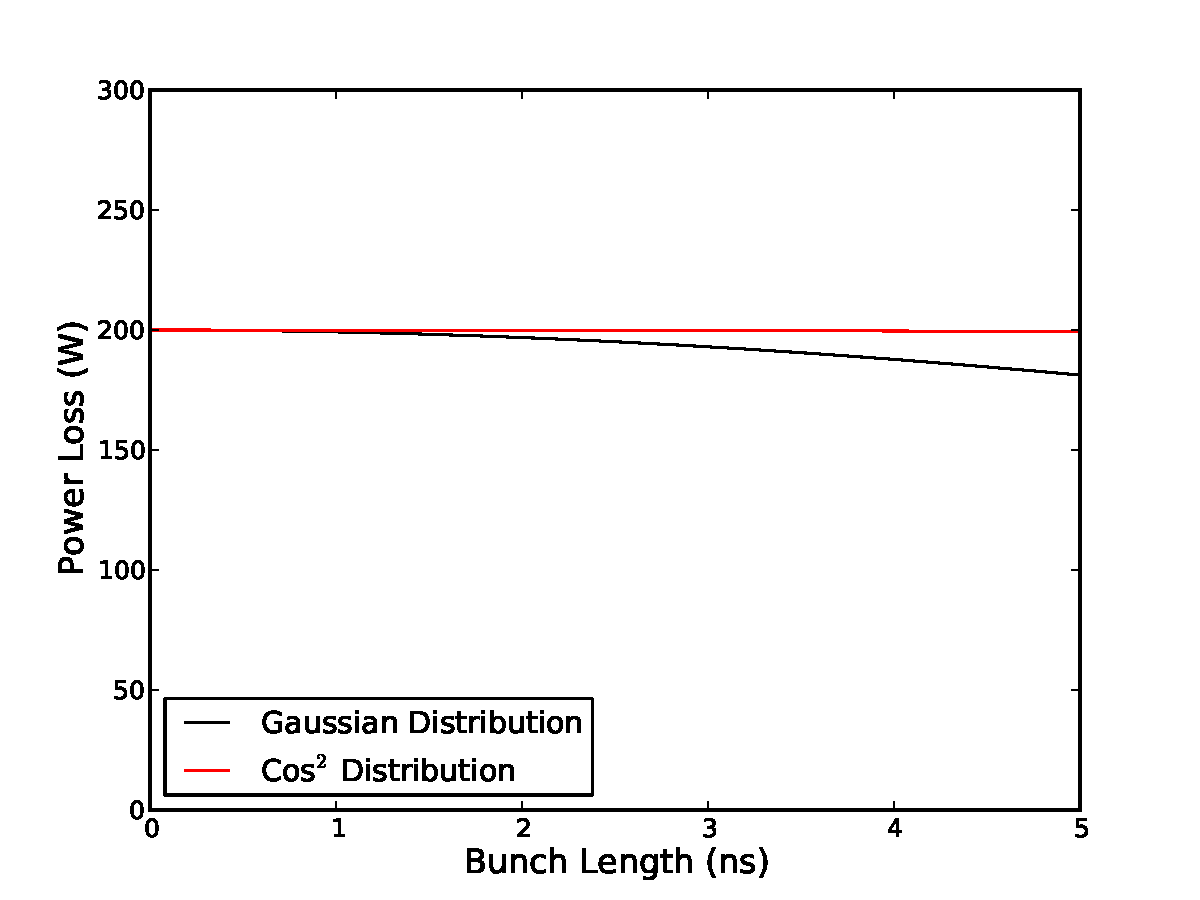
\includegraphics[width=0.5\textwidth]{Wakefields_and_Impedances/figures/heating_broadband_gausscos_bunch_length.pdf}
\label{fig:broadband_heat_bunch_len}
}
\subfigure[]{
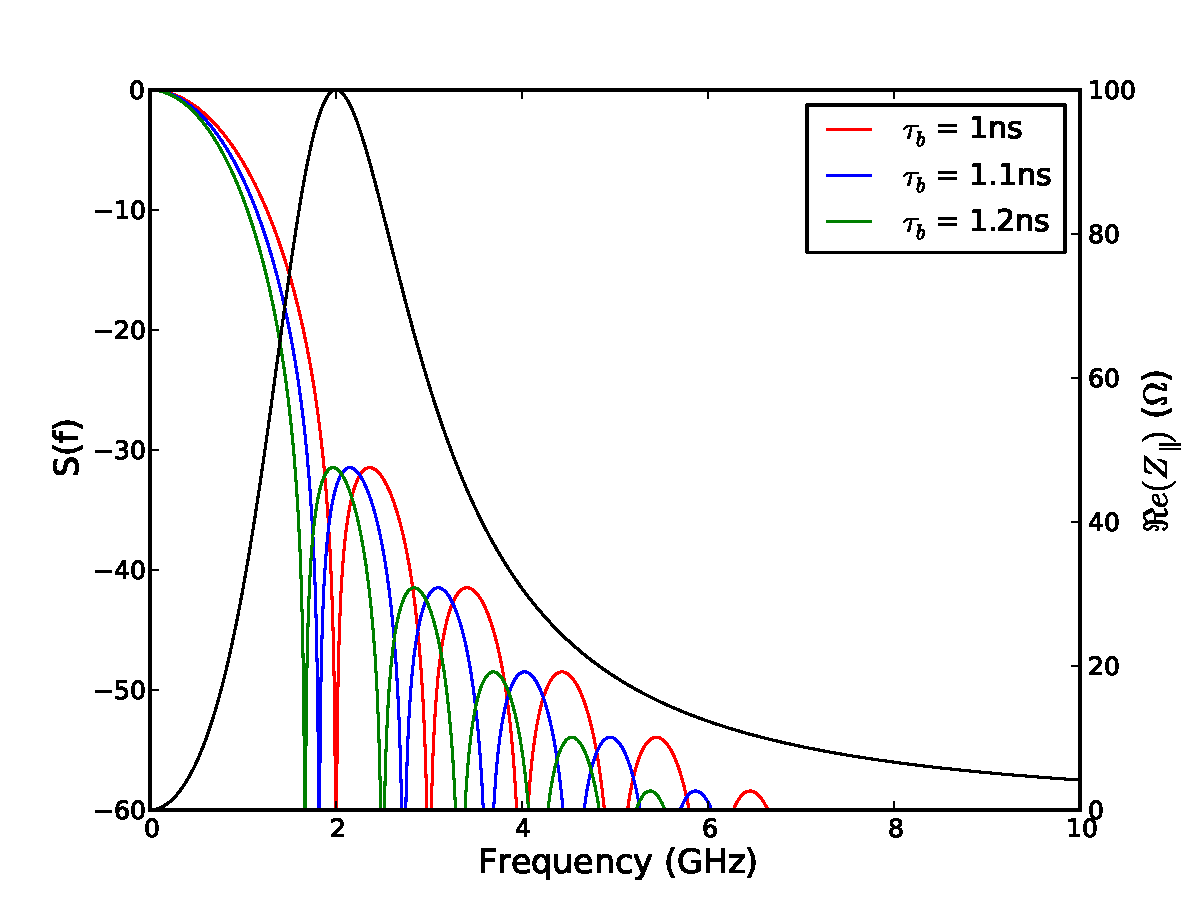
\includegraphics[width=0.5\textwidth]{Wakefields_and_Impedances/figures/impedance_and_power_cos_res_broad.pdf}
\label{fig:broadband_power_loss}
}
\caption{\ref{fig:broadband_heat_bunch_len} The change in power loss due to a narrow band resonance characterised by $\omega_{0} = 2GHz$, $R_{s} = 100\Omega$, $Q = 1$ interacting with a cos$^{2}$ bunch distribution with different bunch lengths. The impedance and the beam power spectrum are shown in \ref{fig:broadband_power_loss} to illustrate how this relates to the power loss.}
\end{figure}

\subsubsection{Beam-Induced Heating due to two traversing beams}

Previous work [cite A. Grudiev TCTVB/TCLIA] has investigated the effect of two beams in a vacuum on the beam-induced heating. This is restated here for the sake of completeness.

To begin, consider the two currents $I_{b1} = I_{0}e^{i\phi_{1}}$ and $I_{b1} = -I_{0}e^{i\phi_{2}}$ representing two counter rotating beams. $I_{0}$ represents the beam current, and $\phi_{1/2}$ the phase of beam 1 and beam 2 respectively. Each beam also sees a seperate potential when it traverses the impedance, given by $V_{b1} = \int_{b1} E_{z} e^{i\omega_{0}z/c} dz$ and $V_{b2} = \int_{b2} E_{z} e^{i\omega_{0}z/c} dz$ respectively. By Ohms law it can then be seen that

\begin{equation}
\begin{pmatrix}
V_{b1} \\
V_{b2}
\end{pmatrix}
=
\begin{bmatrix}
Z_{11} & Z_{12} \\
Z_{21} & Z_{22}
\end{bmatrix}
\begin{pmatrix}
I_{b1} \\
I_{b2}
\end{pmatrix}.
\end{equation}

The power loss due to both beams can then be seen to be

\begin{equation}
P_{loss} = \begin{pmatrix}
V_{b1} & V_{b2}
\end{pmatrix}
\begin{pmatrix}
I_{b1} \\
I_{b2}
\end{pmatrix}^{*}.
\end{equation}

In the worst case scenario, the values of the impedance matrix are real, and are equal in value to the peak values of the resonant impedance
\begin{equation}
Z_{11} = 2R^{b1}_{s};\text{    } Z_{22} = 2R^{b2}_{s};\text{    }  Z_{12} = Z_{21} = 2 \sqrt{R^{b1}_{s}R^{b2}_{s}}.
\end{equation}

The power loss then becomes

\begin{equation}
P_{loss} = I_{0}^{2} 2 \left( R_{s}^{b1} +  R_{s}^{b1} - 2\sqrt{R^{b1}_{s}R^{b2}_{s}} cos \left( \delta \phi \right) \right)
\end{equation}

where $\delta \phi = \phi_{1} - \phi_{2}$ is the phase difference between beam 1 and beam 2. This can be found relatively easy by comparing the distance $\delta s$ from a collision IP of the machine. Assuming the beams are ultrarelativistic $\delta \phi = \omega_{rev} 2  \delta s /c$. It can then be seen that the the last term may either reduce or increase the power loss depending on whether $cos\left( \delta \phi \right) = 1$ or $cos\left( \delta \phi \right) = -1$ respectively.

